\let\negmedspace\undefined
\let\negthickspace\undefined
\documentclass[journal,12pt,onecolumn]{IEEEtran}
\usepackage{cite}
\usepackage{amsmath,amssymb,amsfonts,amsthm}
\usepackage{algorithmic}
\usepackage{graphicx}
\graphicspath{{./figs/}}
\usepackage{textcomp}
\usepackage{xcolor}
\usepackage{txfonts}
\usepackage{listings}
\usepackage{enumitem}
\usepackage{mathtools}
\usepackage{gensymb}
\usepackage{comment}
\usepackage{caption}
\usepackage[breaklinks=true]{hyperref}
\usepackage{tkz-euclide} 
\usepackage{listings}
\usepackage{gvv}                                        
%\def\inputGnumericTable{}                                 
\usepackage[latin1]{inputenc}     
\usepackage{xparse}
\usepackage{color}                                            
\usepackage{array}                                            
\usepackage{longtable}                                       
\usepackage{calc}                                             
\usepackage{multirow}
\usepackage{multicol}
\usepackage{hhline}                                           
\usepackage{ifthen}                                           
\usepackage{lscape}
\usepackage{tabularx}
\usepackage{array}
\usepackage{float}
%\newtheorem{theorem}{Theorem}[section]
%\newtheorem{theorem}{Theorem}[section]
%\newtheorem{problem}{Problem}
%\newtheorem{proposition}{Proposition}[section]
%\newtheorem{lemma}{Lemma}[section]
%\newtheorem{corollary}[theorem]{Corollary}
%\newtheorem{example}{Example}[section]
%\newtheorem{definition}[problem]{Definition}

\begin{document}

\title{5.2.23}
\author{EE25BTECH11020 - Darsh Pankaj Gajare}
% \maketitle
% \newpage
% \bigskip
%\begin{document}
{\let\newpage\relax\maketitle}
%\renewcommand{\thefigure}{\theenumi}
%\renewcommand{\thetable}{\theenumi}
Question:\\
Solve the following system of linear equations
\begin{align}
	\frac{3x}{2} - \frac{5y}{2} = -2, \frac{x}{3} + \frac{y}{2}=\frac{13}{6}
\end{align}
\solution
\begin{table}[H]
	\centering
	\caption{}
	\begin{tabular}{|c|c|}
\hline
\textbf{Name} & \textbf{Value} \\ \hline
$\vec{A}$ & $\myvec{2 & 1 \\0 & 3}$ \\ \hline
\end{tabular}

	\label{}
\end{table}
Let the point of intersection be $\vec{P}$
\begin{align}
	\vec{n_1}^\top\vec{P}=-2
\end{align}
\begin{align}
	\vec{n_2}^\top\vec{P}=\frac{13}{6}
\end{align}
\begin{align}
	\myvec{\vec{n_1}^\top\\\vec{n_2}^\top}\vec{P}=\myvec{-2\\\frac{13}{6}}
\end{align}
\begin{align}
	\augvec{2}{1}{\frac{3}{2} & \frac{-5}{2} & -2\\ \frac{1}{3} &\frac{1}{2} &\frac{13}{6}}
\end{align}
$R_1=2R_1$, $R_2=6R_2$
\begin{align}
	\augvec{2}{1}{3&-5&-4\\2&3&13}
\end{align}
$R_2=R_2-\frac{2}{3}R_1$
\begin{align}
	\augvec{2}{1}{3&-5&-4\\0&\frac{19}{3}&\frac{47}{3}}
\end{align}
\begin{align}
	\frac{19}{3}y=\frac{47}{3} \implies y=\frac{47}{19}
\end{align}
\begin{align}
	3x - 5\cdot\frac{47}{19} = -4 \implies x= \frac{53}{19}
\end{align}
\begin{align}
	\vec{P}=\myvec{\frac{53}{19}\\\frac{47}{19}}
\end{align}
Plot using C libraries:
\begin{figure}[H]
	\centering
	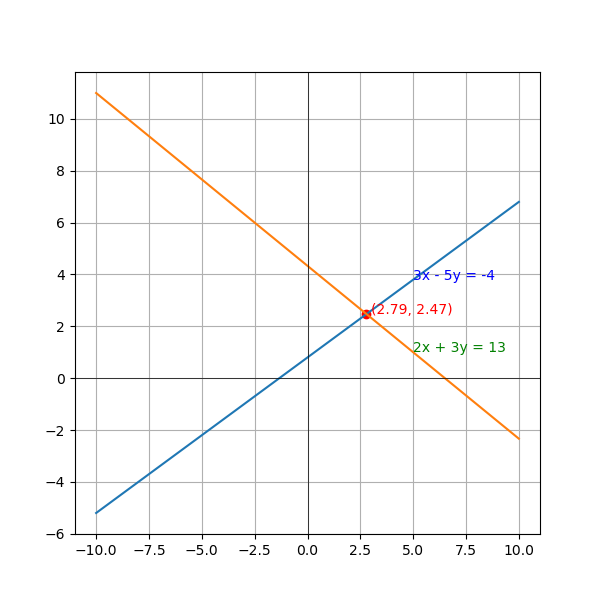
\includegraphics[scale=0.5]{img1}
	\caption*{}
	\label{img1}
\end{figure}
Plot using Python:
\begin{figure}[H]
	\centering
	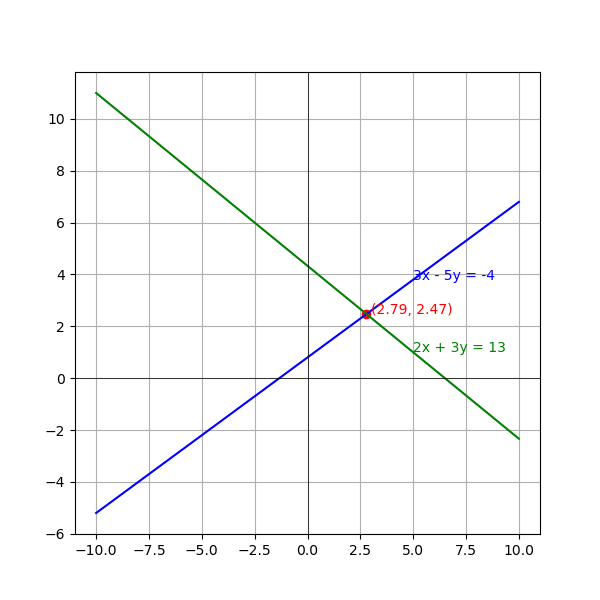
\includegraphics[scale=0.5]{img2}
	\caption*{}
	\label{img2}
\end{figure}
\end{document}

